\chapter{Concept}
\label{ch:Concept}

\abstract{The first section of the third chapter describes the existing application this evaluation is based on. In addition the various phases of the development process are roughly illustrated.
}

\section{Overview of the case study \textit{streets4MPI}}
\label{sec:Concept::Overview}

As stated in~\autoref{sec:Introduction::Goals} the concept for the implementations to compare is inspired by \textit{streets4MPI}, which was implemented to evaluate Python's usefulness for ``computational intensive parallel applications''~\cite[p.3]{streets_report}. It was written by Julian Fietkau and Joachim Nitschke in scope of the module ``Parallel Programming'' in Spring 2012 and makes heavy use of the various libraries of the Python ecosystem. \autoref{fig:architecture_streets4mpi} provides a rough overview about the architecture of \textit{streets4MPI}.

\begin{figure}[htb]
    \centering
    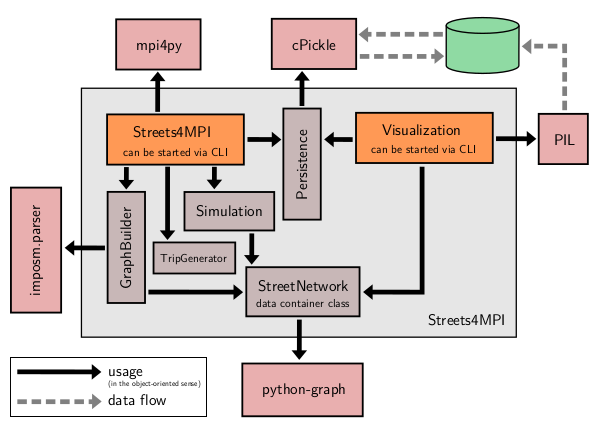
\includegraphics[width=.75\textwidth]{img/architecture_streets4mpi.png}
    \caption{Architecture overview: Streets4MPI~\cite[p. 9]{streets_report}}
    \label{fig:architecture_streets4mpi}
\end{figure}

\textit{streets4MPI} parses \gls{osm} input data, builds a directed graph and repeatedly computes shortest paths for a set amount of ``trips'' (randomly chosen node pairs from the graph) in the graph. Over time it gradually modifies the graph based on results of previous iterations to emulate structural changes in the traffic network in the simulated area. The results can then optionally be written to a custom output format which is visualizable by an additional script~\cite{streets_report}.

As mentioned the applications written in scope of this thesis perform only the graph calculations discarding the produced results. Consequently the implementations do not produce any data besides the runtime statistics externally acquired by benchmark tools.

\section{Differences and limitations}
\label{sec:Concept::Differences}

Although the evaluated implementations are based on the original \textit{streets4MPI}, there are some key implementational differences. This section gives a brief overview over the most important aspects that have been changed and describes both the original application's functionality as well as the derived implementations.

In the remaining part of the thesis the different applications will be referenced quite frequently. For brevity the language implementations to compare will be called by the following scheme: ``streets4<language>''. The Go version for example is called ``streets4go''.

\subsection*{Input format}
\label{subsec:Concept::Differences::Input}

The original \textit{streets4MPI} uses the somewhat dated \gls{osm} \gls{xml} format\fnote{\url{http://wiki.openstreetmap.org/wiki/OSM_XML}} as input which is parsed by \textit{imposm.parser}\fnote{\url{http://imposm.org/docs/imposm.parser/latest/}}. It then builds a directed graph via the \textit{python-graph}\fnote{\url{https://code.google.com/p/python-graph/}} library to base the simulation on~\cite{streets_report}.

The derived versions require the input to be in ``.osm.pbf'' format. This newer version of the \gls{osm} format is based on Google's \gls{protobuf} and is superior to the \gls{xml} variant in both size and speed~\cite{osm_wiki_pbf}. It also simplifies multi language development because the code performing the actual parsing is auto generated from a language independent description file. There are \gls{protobuf} backends for C, Rust and Go which can perform that generation.

\subsection*{Simulation}
\label{subsec:Concept::Differences::Simulation}

The simulation in the base application is based on randomly picked node pairs from the source graph. For these trips the shortest path is calculated by Dijkstra's algorithm as seen in \cite{cormen} and a random factor called ``jam tolerance'' is introduced to avoid oscillation in between iterations~\cite{streets_report}. Then after some time has passed in the simulation, existing streets get expanded or shut down depending on their usage.

The compared implementations of this thesis also perform trip based simulation but without the added randomness and street modification. Also the edge weights are not calculated based on speed limit and length of the street. Instead the derived implementations calculate the length once from the corrdinates of the corresponding nodes and use this as edge weigth directly. The concrete algorithm is a variant of the \shinline{Dijkstra-NoDec} algorithm as seen in~\cite[p. 16]{dijkstra_utcs}. It was mainly chosen because of its reduced complexity in required data structures which again reduces complexity and scope. The algorithm is implemented separately in all three languages so it could theoretically get benchmarked standalone to get clearer results. Mainly because of time constraints this was not attempted in this thesis.

\subsection*{Concurrency}
\label{subsec:Concept::Differences::Concurrency}

\textit{streets4MPI} parallelizes its calculations on multiple processes that communicate via message passing. This is achieved with the aforementioned \textit{MPI4Py} library which delegates to a native \gls{mpi} implementation installed on the system. If no supported implementation is found it falls back to a pure Python solution but the native one should be preferred for maximum performance.

Although Rust as well as Go can integrate decently with existing native code, the reimplementations will be limited to shared memory parallelization on threads. This was mostly decided to evaluate and compare the language inherent concurrency constructs rather than the quality of their foreign funtion interfaces. To achieve a fair comparison \textit{streets4c} will use \textit{OpenMP}~\fnote{\url{http://www.openmp.org}} as it is the de facto standard for simple thread parallelization in C. Of course this solution might not match the performance of hand optimized implementations parallelized with the help of \textit{pthreads} but since the focus is on simple concurrency in the context of scientific applications \textit{OpenMP} was selected as the framework of choice.

\section{Implementation process}
\label{sec:Concept::Implementation}

The implementation process was performed iteratively. Certain milestones were defined and implemented in all three languages. The process only advanced to the next phase when the previous milestone was reached in all applications. This approach was chosen to allow for a fair comparison of the different phases of development. If the implementations would have been developed one after another to completion (or in any other arbitrary order), this might have introduced a certain bias to the evaluation because of possible knowledge about the problem aquired in a previous language translating to faster results in the next one.

\begin{figure}[htb]
    \centering
    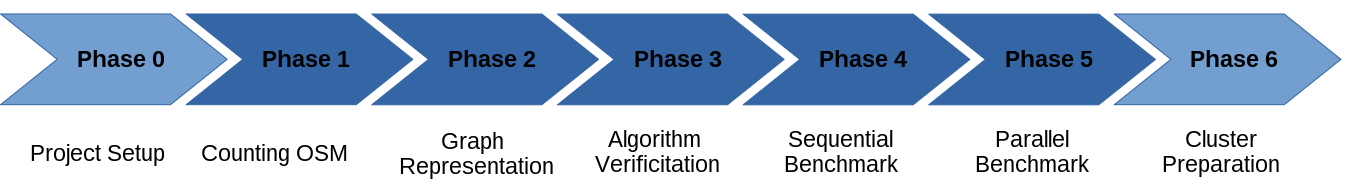
\includegraphics[width=\textwidth]{img/milestone_timeline.png}
    \caption{Milestone overview}
    \label{fig:timeline}
\end{figure}

For each phase various characteristics were captured and compared to highlight the languages' features and performance in the various areas. While the main development and test runs were performed on a laptop the final application was run on a high performance machine provided by the research group Scientific Computing to compare scalability beyond common desktop level processors.

\setcounter{subsection}{-1}

\subsection{Setting up the project}
\label{subsec:Concept::Implementation::Setup}

The first phase of development was to create project skeletons and infrastructure for the future development. The milestone was to have a working environment in place where the sample application could be built and executed. While this is certainly not the most important or even interesting part it did show the differences in comfort between the various toolchains.

\subsection{Counting nodes, ways and relations in an .osm.pbf file}
\label{subsec:Concept::Implementation::Counting}

The first real milestone was to read a .osm.pbf file and count all nodes, ways and relations in it. This was done to get familiar with the required libraries and the file format in general. The time recorded began from the initial project created in phase 0 and finished after the milestone was reached. As this is the most input and output intensive phase it already showed some key differences between the candidates both in speed as well as memory consumption.

\subsection{Building a basic graph representation}
\label{subsec:Concept::Implementation::Graph_Representation}

The next goal was to conceptionally build the graph and related structures the simulation would later operate on. This involved thinking about the relation between edges and nodes as well as the choice of various containers to store the objects efficiently while also keeping access simple. This milestone tested the language's standard libraries and expressiveness in terms of typed containers.

\subsection{Verifying structure and algorithm}
\label{subsec:Concept::Implementation::Verification}

After the base structure to represent graphs and calculate shortest paths was in place it was time to validate the implementations. Unfortunately the OSM data used in the first phase contained too much nodes and ways to be able to efficiently verify any computed results. Therefore a small example graph was manually populated and fed to the algorithm.

\subsection{Benchmarking graph performance}
\label{subsec:Concept::Implementation::SequentialBenchmark}

The fourth milestone was preliminary benchmark of the implementations. The basic idea was to parse the \gls{osm} data used in phase one and build the representing graph. After that the shortest path algorithm is executed once for each node. The total execution time as well as the time taken for each step (building the graph and calculating shortest paths) should be measured and compared as well as the usual memory statistics from previous phases.

\subsection{Benchmarking parallel execution}
\label{subsec:Concept::Implementation::ParallelBenchmark}

The fifth and final phase consisted of modifying the existing benchmark to operate in parallel via threading and benchmarking the results for various configurations. While all the development and previous benchmarks were performed on a personal laptop the final benchmarks were taken on a computation node of the research group to gather relevant results in high concurrency situations.

\subsection{Cluster preperation}
\label{subsec:Concept::Implementation::ClusterPreparation}

\section{Overview of evaluated criteria}
\label{sec:Concept::Criteria}

\begin{itemize}
    \item Performance
    \begin{itemize}
        \item Execution Time
        \item Memory Footprint (consumption total + allocation counts)
    \end{itemize}
    \item Productivity
    \begin{itemize}
        \item \acrshort{sloc} Count
        \item Development Time
        \item Tooling Support
        \item Library Ecosystem
        \item Parallelization Effort
    \end{itemize}
\end{itemize}

\section{Related work}
\label{sec:Concept::Related}

The search for new programming languages which are fit for \gls{hpc} is not a recently developing trend. There have been multiple studies and evaluations but so far none of the proposed languages have gained enough traction to receive widespread adoption. Also most reports focused on the execution performance without really considering additional software metrics or developer productivity~\cite{related_multicore}. at least adds lines of code and development time to the equation but both of these metrics only allow for superficial conclusions about the code quality.

From the candidates presented here Go in particular has been compared to traditional \gls{hpc} languages with mixed results. Although its regular execution speed is somewhat lacking \cite{related_sor_study} showed the highest speedup from parallelization amongst the evaluated languages which is very promising considering high concurrency scenarios like cluster computing. Rust on the other hand has not been seriously evaluated in the \gls{hpc} context probably due to it still being developed.
